\documentclass{beamer}
\usetheme[white]{Wisconsin}
\usepackage{longtable}
\usepackage{listings}
\usepackage{color}
%% The amssymb package provides various useful mathematical symbols
\usepackage{amssymb}
%% The amsthm package provides extended theorem environments
\usepackage{amsthm} \usepackage{amsmath}
%% \usepackage{eqnarray}
\usepackage[mathcal]{euscript} \usepackage{color}
\usepackage{textcomp}
\usepackage{algorithm,algorithmic}
\usepackage[retainorgcmds]{IEEEtrantools}
\usepackage[absolute,overlay]{textpos}
\usepackage{graphicx}
  \setlength{\TPHorizModule}{1mm}
  \setlength{\TPVertModule}{1mm}
\definecolor{listinggray}{gray}{0.9}
\definecolor{lbcolor}{rgb}{0.9,0.9,0.9}
\lstset{
  backgroundcolor=\color{lbcolor},
  tabsize=4,
  rulecolor=,
  language=c++,
  basicstyle=\scriptsize,
  upquote=true,
  aboveskip={1.5\baselineskip},
  columns=fixed,
  showstringspaces=false,
  extendedchars=true,
  breaklines=true,
  prebreak =
  \raisebox{0ex}[0ex][0ex]{\ensuremath{\hookleftarrow}},
  frame=single,
  showtabs=false,
  showspaces=false,
  showstringspaces=false,
  identifierstyle=\ttfamily,
  keywordstyle=\color[rgb]{0,0,1},
  commentstyle=\color[rgb]{0.133,0.545,0.133},
  stringstyle=\color[rgb]{0.627,0.126,0.941},
}

%% colors
\setbeamercolor{boxheadcolor}{fg=white,bg=UWRed}
\setbeamercolor{boxbodycolor}{fg=black,bg=white}

%%----------------------------------------------------------------------------%%
\author{Luke J. Kersting
    \\ NEEP
    \\ University of Wisconsin - Madison
    \\ FRENSIE Meeting
}

\date{\today}
\title{Moment Preserving Monte Carlo Electron Transport}
\begin{document}
\maketitle

%%----------------------------------------------------------------------------%%
\begin{frame}{Outline}

    \begin{itemize}
      \item Monte Carlo Electron Transport
      \item Analog Transport Method
      \item Condensed History Method
      \item Moment Preserving Method
      \item Evaluated Electron Data Library
      \item Implementation
      \item Future Work
    \end{itemize}

\end{frame}

%%----------------------------------------------------------------------------%%
\begin{frame}{Monte Carlo Electron Transport}

  \begin{block}{Challenges}
    \begin{itemize}
      \item Electron charge increases scattering cross section
      \item Neutral Particles may scatter a couple dozen times over a distance
      \item Electrons may scatter 10,000 or more times over the same distance
      \item Purely analog transport is impractical at higher energies
      \item Approximations must be made to reduce computation costs
      \item Monte Carlo development lags behind
    \end{itemize}
  \end{block}
    
  \begin{block}{Motivation}
    \begin{itemize}
      \item Electrons transport needed for precision dose and energy deposition calculations
      \item Photon transport through high Z material
      \item Solid state physics
      \item Medical physics
    \end{itemize}    
  \end{block}  

\end{frame}

%%----------------------------------------------------------------------------%%
\begin{frame}{Condensed History Method}

  \begin{itemize}
    \item ``Condensed'' random walk method to speed up electron transport
    \item Electrons move a set step length that is many mean free paths 
    \item Multiple scattering theory sampled to get the outgoing direction
    \item The Continuous Slowing Down Approximation (CSDA) used to calculate energy loss
    \item Production of secondary particles are averaged
    \item Approximations don't hold below 1 keV
    \item Assumes infinite medium 
  \end{itemize}

\end{frame}

%%----------------------------------------------------------------------------%%
\begin{frame}{Condensed History Step}
  
\begin{figure}
  \centering
  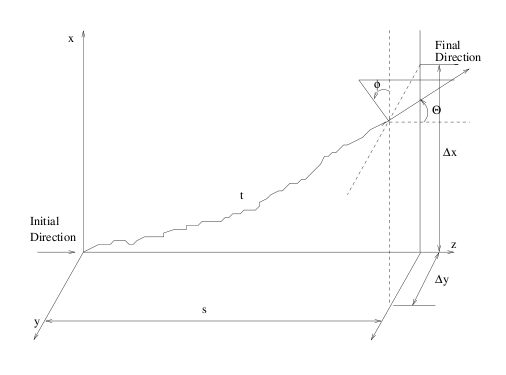
\includegraphics[width=90mm]{electron_step.png}
  \caption{Schematic of electron transport mechanics model in EGS. Where $s$ is the step length, $t$ the total distance traveled, $\Delta x$ and $\Delta y$ are the lateral displacements, $\Theta$ and $\phi$ are the final polar and azimuthal angles.}
\end{figure}


\end{frame}


\end{document}
